\documentclass{nime-alternate}
\usepackage{url}
\usepackage{graphicx, color}
\begin{document}

\numberofauthors{1}
\title{Peacock III: The development of an autonomous non-haptic performance instrument}
\author{
\alignauthor
Chikashi Miyama\\
       \affaddr{College of Music and Dance Cologne}\\
       \email{me@chikashi.net}
}

\maketitle
\begin{abstract}
Peacock III is a box-shaped instrument for musical performances. The instrumemnt is equipped with thirty-five proximity sensors arranged in five rows and seven columns. The sensors detect the movements of a performer's hands and arms in a three-dimensional space above them. In the box, the data from the sensors are collected and digitized by the interface board and send to the main unit, a small embedded computer for the gesture recognition, visualization and sound generation. This paper covers the evolution and the development of the insrtrument.
\end{abstract}

\section{Background and the issues of previous version of Peacock}

\begin{figure}[htbp]
       \begin{center}
              \includegraphics[scale = 0.55]{peacocks.pdf}
       \end{center}
       \caption{Peacock I and II}
       \label{fig:old_peacock}
\end{figure}

Peacock I, The first model of Peacock series, was developed by the author in 2009\cite{miyama:peacock}. Peacock is a musical interface, equipped with 35 infrared proximity sensors that enables a performer to control 35 musical parameters, such as pitch, loudness, and timbre, in realtime without touching or wearing physical devices. Through the musical practice with  Peacock I, several points for improvements were found. 

\begin{enumerate}
\item the bandwidth of the data transfer from the microcontroller to the host computer (ca' 60 Hz.) is not sufficiently high and it produces audience recognizable latency.

\item the infrared sensors employed for Peacock I (Sharp GP2D12), detect the obstacle in the range from 10 to 80 cm. This restrict the performer efficient use of vertical space above the instrument; The use of infrared sensors with longer detection range may enables the performer to control the parameter with higher precision.

\item since the interface should be connected to a host computer by a USB cable to produce sound, a laptop computer must be placed next to the interface. This restricts the autonomy and mobility of the device. 

\item the S/N ratio of the analog data from the infrared sensors is not sufficiently high. The data contain significant amount of analog noise and it disturbs the precise paramter control by the hands.

\item the main circuit board of Peacock I is soldered on a single universal board. Cost and labor reduction for making the device by PCB(printed circuit board) would allow for the creation of multiple Peacock systems in order to realize duo, trio, or ensemble Peacock performances.

\item Peacock I simply detects the distance between 35 infrared sensors and hands and allows one to map these data to musical paramters. However, the recognition of hand position, temporal trajectories, and gestures can be also employed as a certain musical command, if the Peacock recognize it.

\end{enumerate}


In 2011, this project received a DAAD research scholarship and Peacock II, a new version of Peacock, was realized at ZKM, Karlsruhe, Germany. The new version overcame the first three issues mentioned above by using , faster microcontroller\cite{parallax:propeller} and alternative infrared sensors.

Though Peacock II is a significant improvement, there are still four issues for improvement. This paper introduces the features of the newest version of the seires, {\bf Peacock III}, that solve these issues. 

\section{Peacock III}

Peacock III is the newest model of Peacock series, developed in 2014 at KHM, Cologne.

In order to improve the autonomy and mobility of the device, a small computer for the audio synthesis is embedded in the enclosure of Peacock III. It enables users to use Peacock without connecting it to an external laptop for audio synthesis; Peacock III can be used as an autonomous electronic instrument, such as an electric guitar or a keyboard synthesizer. 

Furthermore, a PCB (Printed Circuit Board) is designed as a solution to the fourth and fifth issues. The PCB features denoise the signal from the sensors and it significantly reduces the cost and the labor for the reproduction. 

As a solution to the last issue, a C++ program was developed for gesture recognition; It enables a performer to execute musical commands by moving hands in a certain trajectory above the instrument.

\section{System overview}
\begin{figure}[htbp]
       \begin{center}
              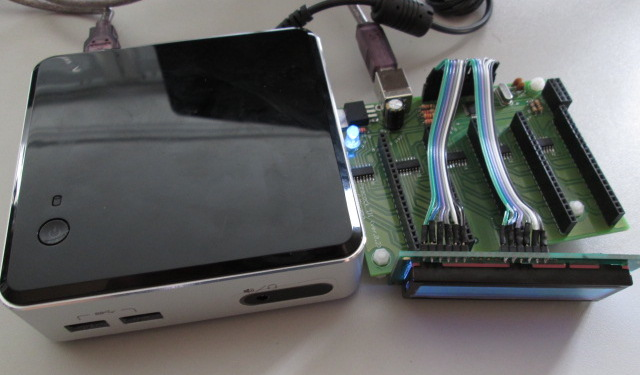
\includegraphics[scale=0.9]{interface_main.jpg}
       \end{center}
       \caption{main unit and interface board}
       \label{fig:interface_main}
\end{figure}

The Peacock hardware consists of two main components;\\
\textbf{main unit} and \textbf{interface board}. The interface board is a 100mm x 60 mm-sized PCB(printed circuit board), that collects the data from all sensors, digitize them, and forward them to the main unit. It is also connected to five buttons and a LCD that enables users to operate the system and indicates the current status of the system.

The main unit, an Intel NUC computer, analyzes the incoming data from the interface board, maps them onto the parameters of software synthesizers, and generates sound. Optionally, the main unit visualizes the incoming data.

\section{Interface Board} % (fold)

\begin{figure}[htbp]
       \begin{center}
              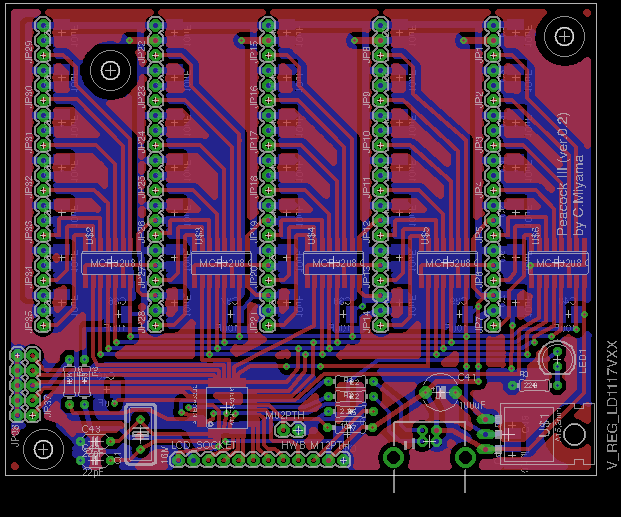
\includegraphics[width=1\columnwidth]{board}
       \end{center}
       \caption{The PCB of Peacock III}
       \label{fig:board}
\end{figure}

The interface board comprises an ATMega 32U2 microcontroller\cite{atmel:avr} and five external 12 bit ADCs, MCP3208, a LCD, 5 buttons and a LED. The main functionalities of the interface board are as follows:

\begin{enumerate}
       \item stabilization of the sensor power supply, employing onboard capacitors.
       \item data collection from the sensors and buttons, employing 5 external ADCs
       \item status indication of the system, using the connected LCD
       \item data transfer to the main unit via a USB cable, employing LUFA framework
\end{enumerate}

\begin{figure}[htbp]
       \begin{center}
              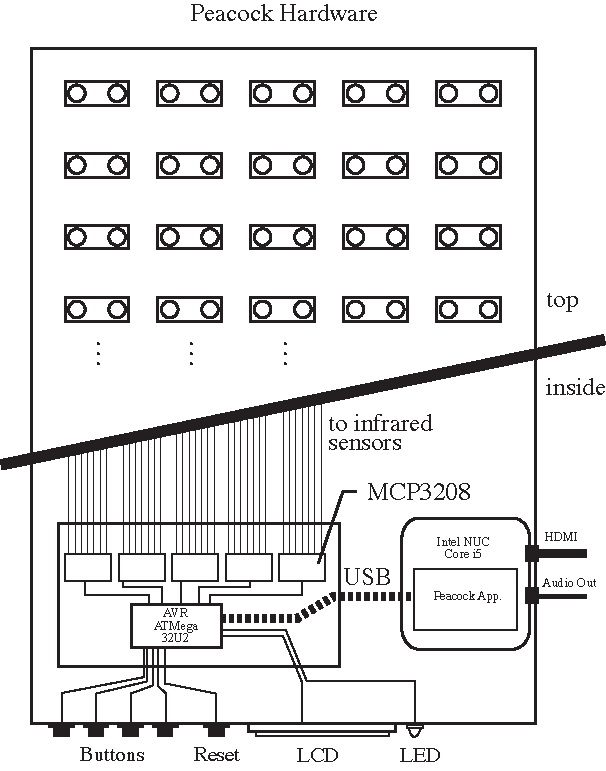
\includegraphics[width=1\columnwidth]{Peacock_hardware.pdf}
       \end{center}
       \caption{The Peacock III Hardware}
       \label{fig:peacock}
\end{figure}

\subsubsection{Hardware signal stabilization} % (fold)
The signal from infrared sensors employed by Peacock include significant amount of noise. In the previous version of Peacock, the signal was denoised in the software by applying digital low pass filters to all incoming digital data. However, The PCB of Peacock III has equiped with capcitor for each infrared sensor for stabilizaing its power supply. Since the cause of noise is mainly by the rapid current draw and pulsations generated by the emitter of the infrared sensor, This hardrware stabilization removes significant amount of noise from the data signal.

\subsubsection{data collection} % (fold)
In order to collect data from all 35 infrared sensors, five 8 channel 12 bit A/D converters(MCP3208) are install on the board and communicates with ATMega 32U2, using SPI(Serial Periferal Interface) protocol. 
The collected data are packed in UART packets with a byte of message ID and check sum.

\subsubsection{Status indication/manipulation} % (fold)

A 2x16 LCD is attached on the side panel of the enclosure and it displays current status of the system. Users are capable of changing the setting of the system, and control the program for the sound synthesis, using buttons, placed next to the LCD.

\subsection{transfer of the data packets} % (fold)

In Peacock I, a FTDI chip bridges the UART messages from the AVR microcontroller to the host computer.
However, by employing AVR ATMega 32U2, a microcontroller with a hardware USB controller, Peacock III is capable of sending data directly from the microcontroller to the host computer. For the development of the USB firmware, the LUFA (Lightweight USB Framework for AVRs)\cite{camera:lufa} was employed. The host computer recognize the Peacock PCB as a virtual serial device( USB CDC class device). The frequency of data transfer is faster than 1000 Hz. The frequency is controlable via the buttons.

\section{Main Unit} % (fold)
A dedicated embedded Intel NUC computer\cite{intel:nuc}, a 101.6 mm x 101.6 mm (UCFF) sized computer with Intel Core i5 processor placed next to the PCB board in the enclosure.

\subsection{Peacock App}
\begin{figure}[htbp]
       \begin{center}
              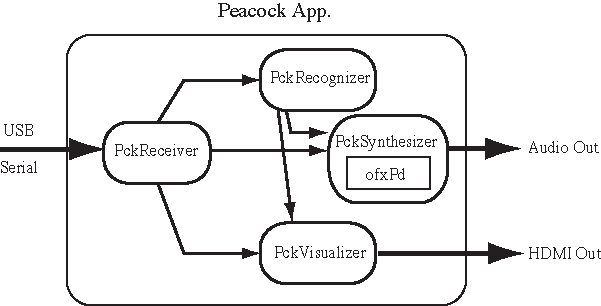
\includegraphics[width=1\columnwidth]{Peacock_app.pdf}
       \end{center}
       \caption{The Peacock III App}
       \label{fig:modules}
\end{figure}

This computer runs Arch linux and {\bf PeacockApp} on it. \\
PeacockApp An openFrameworks\cite{openframeworks}-based application written in C++. This application receives the data from the microcontroller and forwards it to the three sub-modules listed below. 

\begin{enumerate}
       \item Gesture Recognizer(PckRecognizer)
       \item Synthesizer(PckSynthesizer)
       \item Visualizer(PckVisualizer)
\end{enumerate}

In order to minimize the latency and maximize the efficiency of the data processing, These three modules runs on three separate threads in PeacockApp. If the {\it Gesture Recognizer} module detects a certain hand gesture, a notification will be sent immediately to the other two modules.

\subsubsection{Gesture Recognizer: PckRecognizer}

The {\it Gesture Recognizer} modules currently detects, the presence and number of hands above the hardware, estimated position of two hands, centroid of each row and column, the entering points of each hand. 
If this module find some new infomation, notifications to other two modules will be immediately sent.

\subsubsection{Sound Generator: PckSynthesizer}

The sound generator module is programmed with Pd (Pure Data)\cite{Pd}. ofxPd\cite{ofxPd}, an addon of oF\\(OpenFrameworks), enables the PeacockApp to run Pd patches within it. The Pd patches receives all data from the sensors, the result of analysis by the Gesture Recognizer, and the commands from buttons on the side panel. All these data can be mapped to any musical parameters.
 
\subsubsection{Visualizer: PckVisualizer}

Unlike piano, cello, or other acoustic instruments, the player of Peacock controls musical parameters by simply moving hand above the device; There is no physical feedback from the instrument. In order to improve accurate parameter control by the performer, a visualizer is developed.  The visualizer indicates the values of from 35 infrared sensors  the assumed position of hands, chronological trail of hand movement, and recognized gestures, in  3D model programmed with OpenGL\cite{OpenGL}. The renderered 3D images can be displayed by attaching an optional HDMI-compatible monitor to the device.
The visualizer can be deactivated by the user by the attached buttons.
\begin{figure}[htbp]
       \begin{center}
              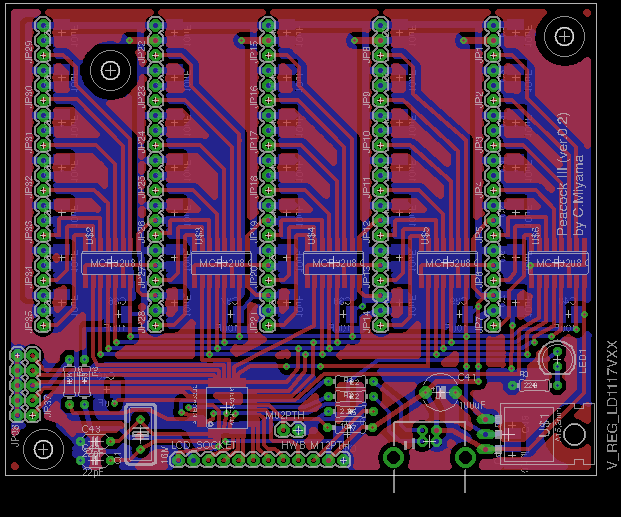
\includegraphics[width=\columnwidth, bb=0 0 621 517]{board.png}
       \end{center}
       \caption{Visualizer}
       \label{fig:visualizer}
\end{figure}


\section{future works}

Further improvement of firmware and in the PeacockApp module is scheduled.
The source code of the PeacockApp and Peacock Firmware is hosted on github.com under GPL v3 lincense.


\section{acknowledgement}
This project is funded by fellowship program of the Academy of Media Arts Cologne. The author would like to express my sincere appreciation to Prof. Anthony Moore and Mr. Dirk Specht for their valuable support.

\bibliographystyle{abbrv}
\bibliography{KHM-references.bib}

\end{document}
